% -*- TeX-master: "main"; fill-column: 72 -*-

\section{Proposed syntax and semantics}
\label{sec:syntax}

In this section, we define the syntax and semantics of the Dynamic Structures package for \sbmlthree. We delineate the data types and constructs defined in this package, then in \sec{sec:examples}, we provide complete examples of using the constructs in example SBML models.

\subsection{Overview of dyn extension}
\label{subsec:overview}

The primary mechanism this package uses to support dynamic cellular behavior are the \Event and \SBase constructs. The Dynamic Structures package extends these components to allow modelers to indicate what cellular processes are being modeled, at which point during simulation (i.e., under what cellular conditions) behaviors happen, and which modeling components are affected by them. To fully enable this, dyn also extends the \Compartment object class to facilitate the representation of spatial rearrangements that follow dynamic cellular processes. Though such representations vary across tools based on the chosen modeling paradigm, this language extension defines the necessary constructs to enable tools to encode dynamic cellular behavior regardless of mathematical method or spatial representation framework.

\subsection{Namespace URI and other declarations necessary for using this package}
\label{subsec:xml-namespace}

Every SBML Level~3 package is identified uniquely by an XML namespace URI.
For an SBML document to be able to use a given SBML Level~3 package, it
must declare the use of that package by referencing its URI.  The following
is the namespace URI for this version of the Dynamic Structures
package for \sbmlthree:

\begin{center}
\uri{http://www.sbml.org/sbml/level3/version1/dyn/version1}
\end{center}

In addition, SBML documents using a given package must indicate whether
understanding the package is required for complete mathematical
interpretation of a model, or whether the package is optional.  This is
done using the attribute \token{required} on the \token{<sbml>} element in
the SBML document.  For the Dynamic Structures package, the value of
this attribute must be set to \val{true}.
The following fragment illustrates the beginning of a typical SBML model
using \sbmlthreecore and this version of the dyn package:

\begin{example}
<?xml version="1.0" encoding="UTF-8"?>
<sbml xmlns="http://www.sbml.org/sbml/level3/version1/core" level="3" version="1"
     xmlns:dyn="http://www.sbml.org/sbml/level3/version1/dyn/version1" dyn:required="true">
\end{example}

\subsection{Primitive data types}
\label{subsec:primitives}
The Dynamic Structures package uses a number of the primitive data types described in Section 3.1 of the \sbmlthreecore specification as well as a number of XML Schema 1.0 data types~\citep{biron:2000}. More specifically, we make use of \primtype{boolean} and \primtype{SIdRef}. This package also adds additional primitive data types described below.

\subsubsection{\emph{Type} \primtype{CBOTerm}}
\label{dat:CBOTerm}

The type \primtype{CBOTerm} is used as the data type of the attribute \token{cboTerm} on the extended \SBase abstract class. \primtype{CBOTerm} follows the syntax defined for the \primtype{anyURI} data type, which considers it a character string data type whose values are interpretable as URIs~(Universal Resource Identifiers; \citep{Means:2001}; \citep{w3c:2000b}) as described by the W3C document RFC 3986 \citep{Berners-Lee:2005}. Examples of valid string values of type CBOTerm are:  
\begin{center}
\url{http://cbo.biocomplexity.indiana.edu/svn/cbo/trunk/CBO_1_0.owl#CellDeath} \url{http://cbo.biocomplexity.indiana.edu/svn/cbo/trunk/CBO_1_0.owl#Movement}
\end{center}
These values are meant to be the identifiers of terms from the Cell Behavior Ontology (CBO) whose curated vocabulary describes cellular entities and processes in computational models. \sec{sec:CBO} provides more information about the ontology, supported ontological terms and general principles for their use in SBML models using this extension.

%\subsubsection{\emph{Type} \primtype{CoordinateSystemKind}}
%\label{dat:CoordSystemKind}
%
%Type \primtype{CoordinateSystemKind} is a primitive data type that is used in extending the \Compartment object to indicate the coordinate system in which the position of modeling elements is to be specified. \primtype{CoordinateSystemKind} is derived from the basic \primtype{XML} type \primtype{string}, but with restrictions about the sequences in which characters may appear. Values for attributes of this data type can only include: \val{cartesian}. The meaning of each of these values is discussed in the context of the extended \Compartment object in \sec{subsec:extCompartment}.
%
%{\color{red} Harold: \notice  If we indicate a coordinateSystem such as cartesian, we should also support other such as "cylindrical", "spherical", and "polar" (which the spatial package also supports). It would make for a more }

\subsubsection{\emph{Type} \primtype{SpatialKind}}
\label{dat:SpatialKind}

The \primtype{SpatialKind} primitive data type is used in the definition of the \SpatialComponent class. \primtype{SpatialKind} is derived from the basic \primtype{XML} type \primtype{string} though it restricts possible values attributes of this data type. Supported values for attributes of this type are bound to a Cartesian coordinate system and include: \val{cartesianX}, \val{cartesianY}, \val{cartesianZ} for describing position in space; \val{alpha}, \val{beta}, and \val{gamma} for describing elemental rotations about the X, Y, and Z coordinate axes (or orientation); and \val{F\textunderscore x}, \val{F\textunderscore y}, and \val{F\textunderscore z} for describing the vector components of the force that drives movement. Attributes of \primtype{SpatialKind} are discussed in the context of the extended \Compartment object in \sec{subsec:extCompartment}.

{\color{red} Harold: \notice The ultimate goal here is to have SpatialKind be of type URI and have values come from an ontology. This means that instead of the allowed values for SpatialKind above, modelers would either use terms from an ontology for characterizing position in space or from CBO- which may potentially be extended to do this. We hope that this will enable modelers to easily describe, for instance, objects modeled in dimensions higher than 3 or objects in vertex-based frameworks}

%Out of the types of off-lattice frameworks, our proposed approach only covers center-based (objects spatially identified by the coordinates of their center of mass) and doesn't support vertex-based (where each object has several vertices that uniquely describe its position)

\subsection{The extended \class{SBase} abstract class}
\label{subsec:extSBase}

The \SBase class is extended in the Dynamic Structures package. As nearly every object composing an SBML Level 3 model has a data type that is derived directly or indirectly from \SBase, the addition of a \token{cboTerm} attribute enables modelers to attach cell-behavior specific ontological terms to each major element or list in an SBML model. \ref{fig:UMLExtendedSBase} provides the corresponding UML diagram of the extended \SBase class. 

%The \SBase class is extended in the Dynamic Structure package. The addition of a \token{cboTerm} attribute is designed to allow a modeler or a software package to attach semantical information to \Event objects triggered to model dynamic cellular processes. As nearly every object composing an SBML Level 3 model has a data type that is derived directly or indirectly from \SBase, extending this base type enables modelers to attach ontological information to each major element or list in an SBML model.

\begin{figure}[tbhp]
	\centering
	%\usepackage{graphicx}
	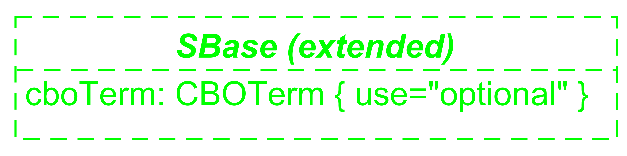
\includegraphics[width=0.32\textwidth]{images/UMLExtendedSBase.pdf}\\
	\caption{A UML representation of the extended \SBase abstract class. See \ref{subsec:conventions} for conventions related to this figure.} \label{fig:UMLExtendedSBase}
\end{figure}

\subsubsection{The \token{cboTerm} attribute}
\label{attr:cboTerm}

The attribute called \token{cboTerm} on the \SBase abstract class supports the use of Cell Behavior Ontology(CBO) terms on most SBML components. The relationship is of the form "an SBML component is-a X", where X is the CBO term. The term chosen should be the most precise one that captures the role of the component in the model. The value of \token{cboTerm} must conform to the syntax permitted by the \primtype{CBOTerm} data type previously described in \sec{dat:CBOTerm} of the current specification. The scope of the \token{cboTerm} attribute is local to the enclosing object definition and is not visible outside the object definition. 

As described in \sec{subsec:extEvent}, though nearly all SBML components may define values for this attribute, special focus is placed on \Event constructs. For a discussion on supported values for \token{cboTerm} on particular SBML objects and CBO in general, see \sec{sec:CBO}.


\subsection{The extended \class{Event} object}
\label{subsec:extEvent}

The \Event class is extended in the Dynamic Structures package. Adding a value for the \SBase-inherited \token{cboTerm} attribute allows a modeler, or a software package, to attach semantical information to events triggered to model dynamic cellular processes. The \token{applyToAll} attribute and subobjects \ListOfDynElements and \DynElement allow modelers to indicate which SBML components are involved in a given \Event. \ref{fig:UMLExtendedEvent} provides the corresponding UML diagram. 

\begin{figure}[tbhp]
  \centering
  %\usepackage{graphicx}
  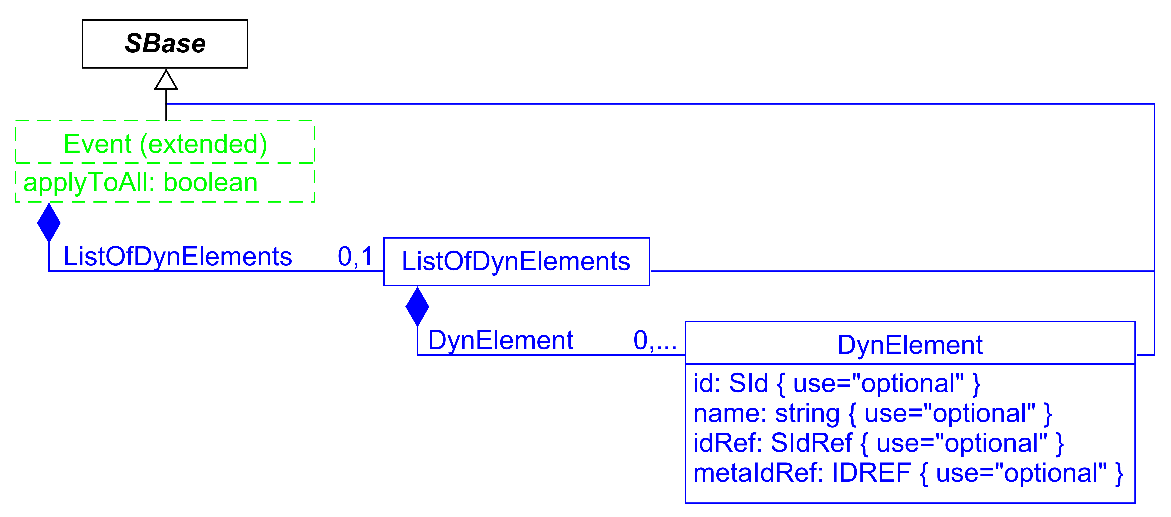
\includegraphics[width=0.75\textwidth]{images/UMLExtendedEvent.pdf}\\
  \caption{A UML representation of the extended \Event class and newly defined \ListOfDynElements and \DynElement objects. See \ref{subsec:conventions} for conventions related to this figure.} \label{fig:UMLExtendedEvent}
\end{figure}

\subsubsection{The \token{applyToAll} attribute}
\label{attr:applyToAll}
The \token{applyToAll} attribute is used as a mechanism for indicating which SBML model components are impacted by the execution of the current dynamic \Event. If the value of this attribute is \val{true}, then all SBML elements in the model are involved in the \Event. If \val{false}, modelers must list the specific components that are affected by means of the \ListOfDynElements class. For instance, if the value of the \token{cboTerm} attribute semantically annotates the current \Event as modeling cell death, the \token{applyToAll} attribute allows modelers to chose whether only some or all of the model components are to be removed from the simulation. 

\subsubsection{The \class{ListOfDynElements} class}
\label{subsec:ListOfDynElements}
An extended \Event component with \val{false} as value for its \token{applyToAll} attribute must define an object of class \ListOfDynElements. This object contains a list of \DynElement references that uniquely identify the set of SBML components involved in the execution of a given dynamic \Event.

\subsection{The \class{DynElement} class}
\label{subsec:DynElement}
A \DynElement object contains unique references to SBML components defined within a model. These references are pooled by a \ListOfDynElements construct and modified characteristically depending on the cellular process that is modeled. This construct contains two optional attributes, \token{id} and \token{name}, which allow others to reference it. \DynElement also defines two optional attributes, \token{idRef} and \token{metaIdRef}, which serve to store a reference to a given SBML component in the model. It is important to note that exactly one (and only one) of these attributes (\token{idRef} and \token{metaIdRef}) must have a value in a given \DynElement object instance, and that references are not permitted to be circular: no \DynElement may reference itself, its parent \ListOfDynElements, nor its parent \Event.

\subsubsection{The \token{id} and \token{name} attributes}
\label{attr:idNameDynElement}

The optional \token{id} attribute serves to provide a way to reference \DynElement objects from elsewhere in the model.
The attribute takes a value of type \primtype{SId}. Note that the identifier of a \DynElement reference carries no mathematical
interpretation and cannot be used in mathematical formulas in a model. \DynElement also carries an optional \token{name}
attribute, which is of type \primtype{string}. The \token{name} attribute may be used in the same manner as other name attributes on \sbmlthreecore objects; please refer to Section~3.3.2 of the \sbmlthreecore specification for more information.

\subsubsection{The \token{idRef} attribute}
\label{attr:idRef}

The \token{idRef} is an optional attribute of the type \primtype{SIdRef} that must be defined if a \DynElement has no defined \token{metaIdRef} attribute, and must not be defined otherwise. This attribute is used to reference single anatomical structures (compartments or submodels) or additional SBML components that are altered following the execution of a given dynamic event. Only model elements having identifiers of type \primtype{SId} can be referenced by this attribute. 

The namespace in which the \primtype{SId} is to be found is the \primtype{SId} namespace of the \Model to which the \DynElement belongs. This includes elements from SBML packages which may have elements with id values that are part of the \primtype{SId} namespace of the \Model, such as \class{Deletion} elements from the Hierarchical Model Composition package, \class{FluxBound} elements from the Flux Balance Constraints package, and \class{Group} and \class{Member} elements from the Groups package. Conversely, elements with id values that are not part of the \primtype{SId} namespace of the \Model such as \UnitDefinition and \LocalParameter elements in \sbmlthreecore, or \class{Port} elements from the Hierarchical Model Composition package, may not be referenced by this \token{idRef} attribute.

When \token{idRef} points to \Compartment element, it is advisable to define a \ListOfSpatialComponents object as seen in \ref{subsec:extCompartment}. This ensures that when an extended \Event is executed, referenced cellular compartments will have an assigned spatial description, which is important in representing dynamic behavior. On the other hand, if this attribute points to the identifier of a \class{Group} from the SBML Groups extension, the \DynElement references not the \class{Group} element, but all the elements within instead. For a complete description of how \DynElement class instances are affected by different behaviors modeled in an extended \Event, refer to \sec{subsubsec:supportedCBO}.

\subsubsection{The \token{metaIdRef} attribute}
\label{attr:metaIdRef}

The \token{metaIdRef} is an optional attribute of the type \primtype{IDREF} that must be defined if a \DynElement has no defined \token{idRef} attribute, and must not be defined otherwise. This attribute is used to reference single anatomical structures (compartments or submodels) or additional SBML components that are altered following the execution of a given dynamic event. This attribute points to the \token{metaid} attribute value of other objects in the \Model and should be used in cases where the object being referenced does not have an identifier in the \Model \primtype{SId} namespace, which is the case of the \UnitDefinition and \LocalParameter elements in \sbmlthreecore.

Since meta identifiers are optional attributes of \SBase, all SBML objects have the potential to have a meta identifier value, including most elements from other SBML packages. Note that even if used in conjunction with the Hierarchical Model Composition package, this attribute is not allowed to reference elements from other \Model objects in the same SBML document. Moreover, as in the case of \token{idRef}, if \token{metaIdRef} points to \Compartment element, it is advisable to define a \ListOfSpatialComponents object as explained in \ref{subsec:extCompartment}.

\subsection{The extended \class{Compartment} object}
\label{subsec:extCompartment}

The \Compartment class may be extended to represent the spatial location and subsequent rearrangement that follows dynamic cellular processes emulated by extended \Event constructs. Refer to \sec{sec:CBO} for a list of supported dynamic cellular processes and associated ontological terms. This SBML extension adds to \Compartment the subobjects \ListOfSpatialComponents and \SpatialComponent to describe the location and orientation of cellular components as well as how they move in space. \ref{fig:UMLExtendedCompartment} provides the corresponding UML diagram of the various features of the extended \Compartment class. 

\begin{figure}[tbhp]
	\centering
	%\usepackage{graphicx}
	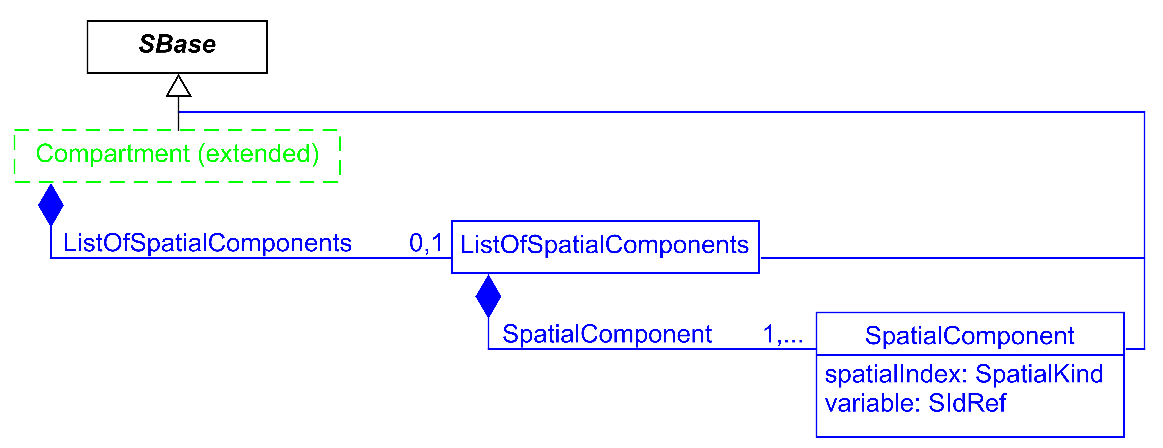
\includegraphics[width=0.85\textwidth]{images/UMLExtendedCompartment.pdf}\\
	\caption{UML diagram for the extension of the \Compartment object and the definition of \ListOfSpatialComponents and \SpatialComponent classes. See \ref{subsec:conventions} for conventions related to this figure.} \label{fig:UMLExtendedCompartment}
\end{figure}

\subsubsection{The \class{ListOfSpatialComponents} class}
\label{subsec:listSpatialComp}

\Compartments mapped by a \DynElement construct may contain a listOfSpatialComponents element, of class \ListOfSpatialComponents. Each list contains \SpatialComponent objects that together serve to describe the spatial location (center of mass), orientation (Euler angles) and force vector (in the case of movement) of a given \Compartment. If mapped, a \Compartment cannot have an empty \ListOfSpatialComponents list.

\subsection{The \class{SpatialComponent} class}
\label{subsec:spatialComp}

Instances of the \SpatialComponent class may represent individual components of either the spatial location, orientation or force vector of mapped \Compartment structures that are involved in dynamic events. To this end, this construct defines two mandatory attributes: \token{spatialIndex} and \token{variable}. Being derived from \SBase, this class also has all the usual attributes and elements of its parent class.

\subsubsection{The \token{id} and \token{name} attributes}
\label{attr:idNameSpatialComp}

The optional \token{id} attribute serves to provide a way to reference \SpatialComponent objects from elsewhere in the model.
The attribute takes a value of type \primtype{SId}. Note that the identifier of a \SpatialComponent reference carries no mathematical
interpretation and cannot be used in mathematical formulas in a model. \SpatialComponent also carries an optional \token{name}
attribute, which is of type \primtype{string}. The \token{name} attribute may be used in the same manner as other name attributes on \sbmlthreecore objects; please refer to Section~3.3.2 of the \sbmlthreecore specification for more information.

\subsubsection{The \token{spatialIndex} attribute}
\label{attr:spatialIndex}

The attribute \token{spatialIndex} of type \primtype{SpatialKind} is added to uniquely identify individual components of either the spatial location, orientation or force vector of an object modeled in a Cartesian coordinate system. \token{SpatialIndex} may take one of all the possible \primtype{SpatialKind} values specified in \sec{dat:SpatialKind}. A single \val{cartesianX} \SpatialComponent can be used to define one-dimensional systems; two-dimensional systems are in turn characterized by having two \SpatialComponent children with \token{spatialIndex} values of \val{cartesianX} and \val{cartesianY}; and three-dimensional ones can be defined by having three \SpatialComponent elements with \token{spatialIndex} values of \val{cartesianX}, \val{cartesianY}, and \val{cartesianZ}. Rotational angles along X, Y and Z coordinate axes (orientation) may be defined by having \SpatialComponent elements with respective \token{spatialIndex} values of \val{alpha}, \val{beta}, and \val{gamma}. Finally, values such as \val{F\textunderscore x}, \val{F\textunderscore y}, and \val{F\textunderscore z} for \token{spatialIndex} can be used to describe the X, Y, and Z vector components of the force that characterizes object movement in space.
 
\subsubsection{The \token{variable} attribute}
\label{attr:variable}

The \token{variable} attribute of type \primtype{SIdRef} contains the identifier of a \Parameter defined in the model that serves to quantitatively specify an object's position, orientation or force components. The scope of the referenced \Parameter component must be global to the whole model and its \token{constant} attribute must be set to \val{false} as the spatiality of the associated \Compartment may change in response to dynamic processes.
